\documentclass{report}
\usepackage{graphicx} % Required for inserting images
\usepackage[italian]{babel}
\usepackage{tikz}
\usepackage{hyperref}
\usepackage{amsmath}
\usepackage{xcolor}
\usepackage{float}

\definecolor{darkgreen}{rgb}{0.0, 0.5, 0.0}


\title{Riconoscimento tramite Voce, Firma e Retina}
\date{Parte VIII}

\begin{document}

\maketitle

\tableofcontents
\newpage

\chapter{Sistemi basati sul riconoscimento vocale}

Il riconoscimento biometrico della voce è considerato tecnicamente un \textbf{ibrido} tra biometria fisiologica e
comportamentale, dal momento che l’emissione è determinata non solo dalla conformazione della gola e della
laringe, ma anche da \textbf{aspetti comportamentali} dell'utente, quali ad esempio il proprio tono umorale.

\noindent Fino ad oggi il riconoscimento vocale avviene in 3 modalità:
\begin{itemize}
    \item auditivo (un esperto ascolta due tracce vocali e le identifica)
    \item semiautomatico (un esperto controlla delle feature estratte dalla voce di 
    di due persone, come spettogrammi o lunghezze d'onda)
    \item completamente automatico
\end{itemize}


\section{Introduzione}

L'acquisizione può avvenire:
\begin{itemize}
    \item Con un semplice microfono
    \item Telefono
    \begin{itemize}
        \item Aumentà la fruibilità ma rende il processo biometrico più complesso, a causa 
        della riduzione di informazioni dovuta alla \textbf{limitata banda destinata alla voce su linea telefonica}
    \end{itemize}
    \item Cooperativa 
    \begin{itemize}
        \item Registrazione da parte dell'utente di una frase predefinita per un certo numero di volte (ad esempio una sequenza di numeri)
        \item \textbf{Text dependent:} è noto il parlato, tutti gli individui che fanno l'enrollment dicono la stessa frase 
        \item \textbf{Text independent:} non si conosce nulla del parlato 
    \end{itemize}
    \item Non cooperativa 
    \begin{itemize}
        \item L'identificazione avviene senza che l'interessata ne sia a conoscenza (ambito investigativo)
    \end{itemize}
\end{itemize}

\subsection{Text Dependent e Text Independent}
\begin{itemize}
    \item \textbf{Text Dependent}
    
    \textcolor{darkgreen}{\textbf{+}} sample più brevi

    \textcolor{darkgreen}{\textbf{+}} protegge meglio la privacy

    \textcolor{red}{\textbf{-}} serve cooperazione dell'utente 
    \item \textbf{Text Independent}
    
    \textcolor{red}{\textbf{-}} sample più lunghi

    \textcolor{darkgreen}{\textbf{+}} usato in una normale conversazione

    \textcolor{darkgreen}{\textbf{+}} non serve cooperazione
\end{itemize}

\section{Caratteristiche generali della voce}
L'elaborazione della traccia acustica riflette:
\begin{itemize}
    \item Anatomia (dimensione e conformazione di gola e bocca)
    \item Comportamento (timbro di voce, modo di parlare)
\end{itemize}

\begin{figure}[ht]
    \centering
    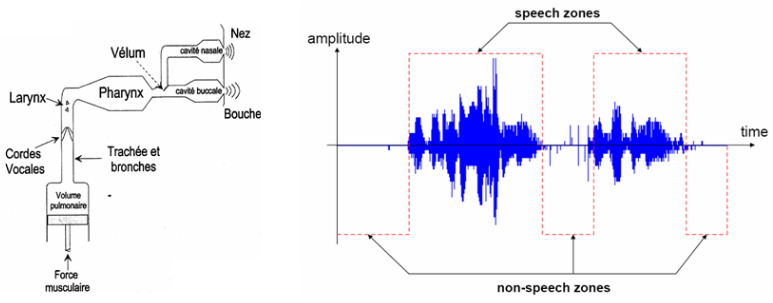
\includegraphics[width=1\linewidth]{images/voce-char.png}
\end{figure}

\newpage
\noindent Si possono estrarre diverse caratteristiche:
\begin{itemize}
    \item \textbf{Alto livello:} caratteristiche sintattiche e lessicali
    \item \textbf{Livello intermedio:} qualità della voce 
    \item \textbf{Basso livello:} energia del suono nelle bande spettrali
\end{itemize}

\section{Estrazione e matching}
I passi principali effettuati sono:
\begin{enumerate}
    \item \textbf{Prefiltraggio}
    \item \textbf{Elaborazione delle feature} statiche e dinamiche 
    \item \textbf{Modellazione} del parlatore 
    \item \textbf{Comparazione} dei modelli e decisione
\end{enumerate}

\section{Vantaggi e Svantaggi}
\begin{itemize}
    \item \textcolor{darkgreen}{\textbf{Vantaggi}}
    \begin{itemize}
        \item Tecnologia basata su hardware di larga diffusione 
        \item Buona accettabilità da parte degli utenti 
    \end{itemize}
    \item \textcolor{red}{\textbf{Svantaggi}}
    \begin{itemize}
        \item Possibili lunghi tempi per enrollment
        \item Elevate dimensioni del template (1 MB)
        \item Sensibilità a rumori di fondo 
        \item Variabilità intraclasse dovuta a malattie o condizioni ambientali 
        \item Facile falsificazione del tratto
    \end{itemize}
\end{itemize}

\chapter{Riconoscimento biometrico della firma}
La firma è unica non solo visivamente ma anche per una serie di caratteristiche;
se viene usata una tavoletta, è possibile trasformare tali aspetti in dati.

\section{Acquisizione della firma}

\subsection{Firma online}
Valuta una serie di parametri, tra cui:
\begin{itemize}
    \item velocità di scrittura
    \item punti nei quali si esercita più pressione 
    \item angolo d'inclinazione della penna 
    \item accelerazione del movimento 
    \item numero di volte che la penna viene sollevata
\end{itemize}

\noindent Vengono inoltre:
\begin{itemize}
    \item Misurati dei tracciati dei parametri nel tempo (distanze relative spazio-temporali di punti singolari)
    \item Punti singolari dei tracciati (inversioni di moto, intersezioni delle linee)
\end{itemize}

\begin{figure}[H]
    \centering
    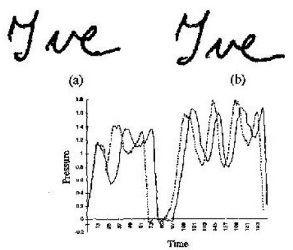
\includegraphics[width=0.5\linewidth]{images/firma-online.png}
\end{figure}

\subsection{Firma offline}
In questo caso non sono dati i parametri di esecuzione della firma nel tempo, ma è solo a disposizione l’immagine
della firma come sample iniziale.

Il confronto, in questo caso, avviene:
\begin{itemize}
    \item con gli istogrammi delle proiezioni orizzontali e verticali dei toni di grigio
    \begin{figure}[ht]
        \centering
        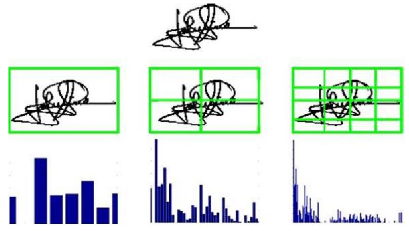
\includegraphics[width=0.55\linewidth]{images/isto.png}
    \end{figure}
    \item \textit{Extended Shadow Code:} tecnicha che permette di codificare 
    la firma in un codice sovrapponendo una serie di matrici di segmenti sulla firma, 
    e verificando le intersezioni 
    \begin{figure}[ht]
        \centering
        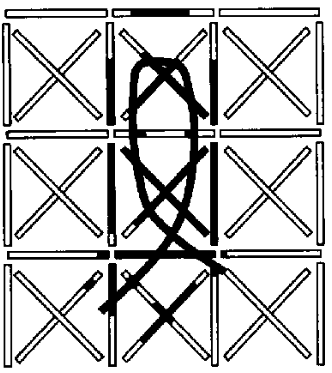
\includegraphics[width=0.3\linewidth]{images/shadow.png}
    \end{figure}
\end{itemize}

\section{Vantaggi e Svantaggi}
\begin{itemize}
    \item \textcolor{darkgreen}{\textbf{Vantaggi}}
    \begin{itemize}
        \item hardware poco costoso
        \item buona accettabilità da parte degli utenti 
        \item difficilmente falsificabile (firma online)
    \end{itemize}
    \item \textcolor{red}{\textbf{Svantaggi}}
    \begin{itemize}
        \item instabilità temporale del campione (variabilità intraclasse)
        \item dimensioni del template (fino 1,5MB per scansioni)
        \item numero limitato di applicazioni adatte
        \item similitudine interclasse per firme troppo brevi o semplici
    \end{itemize}
\end{itemize}


\chapter{Riconoscimento biometrico della retina}

Nei sistemi per il riconoscimento delle persone basati su immagini della retina i sensori acquiscono il particolare
pattern dei vasi presenti sulla retina:
\begin{itemize}
    \item il pattern è già completo alla nascita e rimane quasi completamente stabile per 
    tutta la durata della vita 
    \item La distribuzione sulla retina dei vasi è casuale e univoca
\end{itemize}

\begin{figure}[ht]
    \centering
    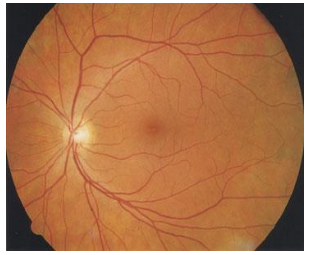
\includegraphics[width=0.7\linewidth]{images/retina.png}
\end{figure}

\newpage
\section{Acquisizione ed estrazione di caratteristiche}
\begin{itemize}
    \item Il sensore deve essere posizionato a breve distanza 
    dall'occhio per avere una corretta acquisizione del tratto 
    \item Con metodi simili a quelli delle impronte digitali vengono 
    ricercate le minutiae e memorizzate in un template 
\end{itemize}

\begin{figure}[ht]
    \centering
    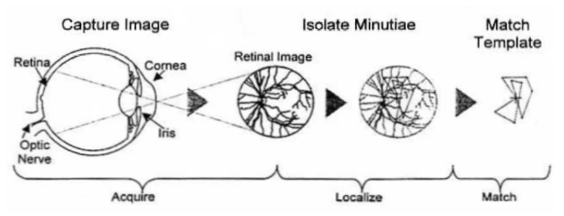
\includegraphics[width=1\linewidth]{images/iride-acqusizione.png}
\end{figure}

\section{Vantaggi e Svantaggi}
\begin{itemize}
    \item \textcolor{darkgreen}{\textbf{Vantaggi}}
    \begin{itemize}
        \item efficiente 
        \item stabile 
        \item difficile da falsificare 
        \item difficilmente alterabile da fattori esterni 
    \end{itemize}
    \item \textcolor{red}{\textbf{Svantaggi}}
    \begin{itemize}
        \item difficilmente applicabile in applicazioni commerciali 
        \item percepito dagli utenti come intrusivo
        \item percepito come pericoloso per la vista 
        \item elevato costo dei sensori
    \end{itemize}
\end{itemize}



\end{document}